\documentclass[a4paper]{exam}

\usepackage{graphicx}

\usepackage{siunitx}
\DeclareSIUnit{\revolution}{rev}
\DeclareSIUnit{\rpm}{\revolution\per\minute}
\DeclareSIUnit{\lightyear}{ly}

\begin{document}
  \section*{L2 Physics: Problems on waves}
  The speed of sound is \SI{340}{\metre\per\second} in air. See also the final page for useful formulae.
  \subsection*{Sections 1.1-1.2}
  \begin{questions}
    \question A radio station sends out radio waves with frequency \SI{750}{\kilo\hertz}. All radio waves travel with a speed
              of \SI{3.0e8}{\metre\per\second}. How far apart are the crests of the wave sent out by the station?
    \question A television station sends out radio waves with frequency \SI{750}{\mega\hertz}. All radio waves travel with a speed
              of \SI{3.0e8}{\metre\per\second}. How far apart are the crests of the wave sent out by the station?
    \question A wave has wavelength \SI{2}{\centi\metre}; at a given point, 25 wave crests per second are observed. Calculate
              (a) the frequency of the wave; (b) the speed of the wave; (c) the time between observed wave crests.
    \question The wave shown below is travelling to the right with a speed of \SI{2.00}{\metre\per\second}. How long
              after the instant shown will the crest on the left have moved to the position of the crest on the right?

              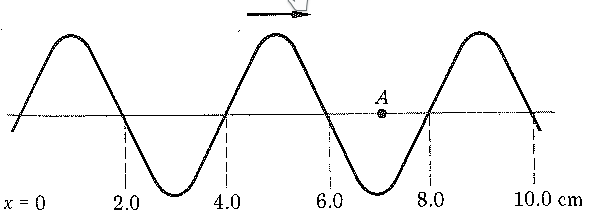
\includegraphics[width=0.4\textwidth]{beuche132}
    \question If the same wave is slowed so that it is moving at a speed of \SI{100}{\centi\metre\per\second}, how many
              crests per second will pass point $ A $?
    \question What frequency must a sound source have if the wavelength of its sound is to be \SI{3.0}{\centi\metre}?
  \end{questions}
  \subsection*{Sections 1.3-1.4}
  \begin{questions}
    \question The two pulses in the igure are moving down the string at \SI{2.0}{\metre\per\second} each. Sketch the position
              of the string (a) after \SI{0.40}{\second}; (b) after \SI{0.20}{\second}.

              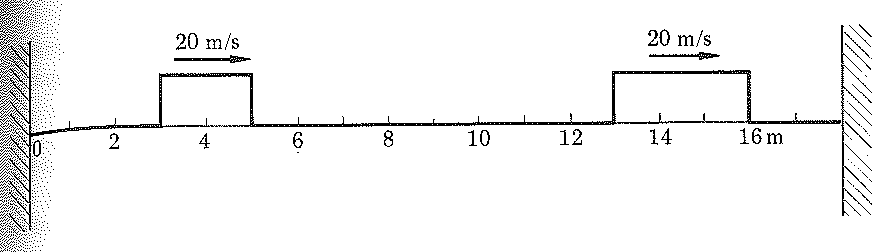
\includegraphics[width=0.4\textwidth]{beuche131}
    \question Two waves moving in opposite directions can interfere with each other in such a way that no net movement is seen;
              this is called an \emph{standing wave}. Give a simple example of an experiment you could set up to show this.
    \question Describe a water-wave experiment which illustrates the phenomenon of diffraction.
    \question Jenna is conducting an experiment; she places a tone generator (a machine that generates a particular frequency
              of wave) on the other side of a narrow slit in a sound-proof barrier. She notices that, if the generator is placed
              around the corner as in the following diagram, the sound of the generator is much louder when it is set to a lower
              frequency. Explain this observation.

              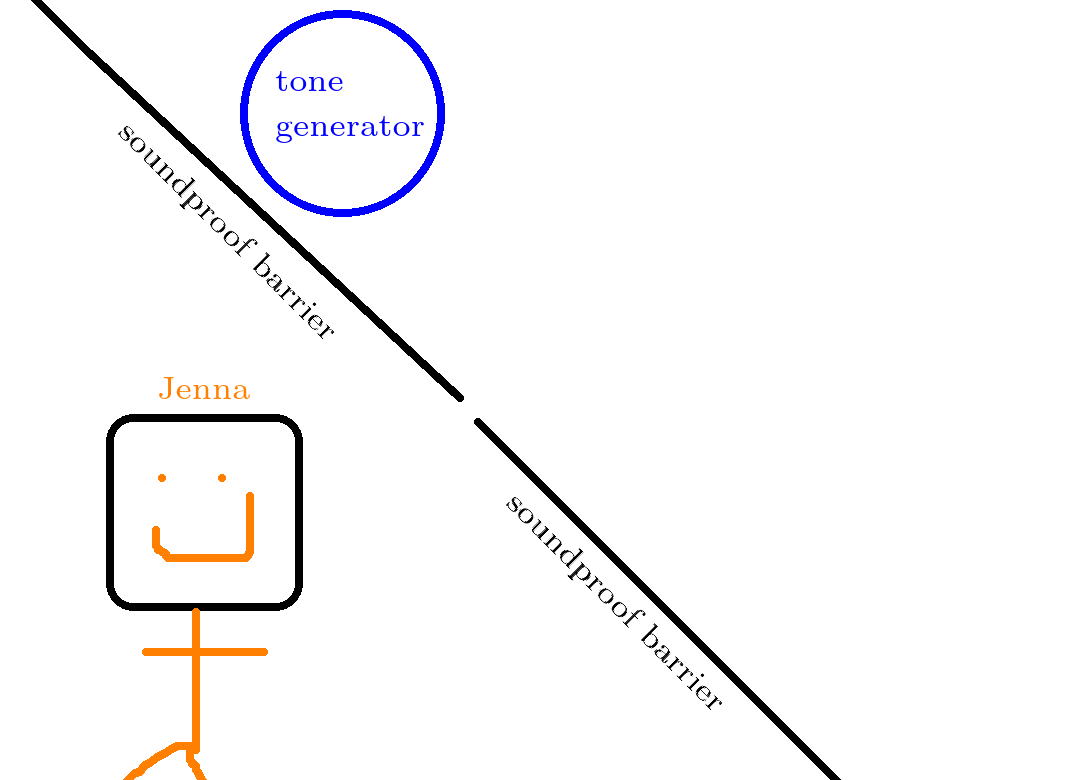
\includegraphics[width=0.4\textwidth]{jenna}
    \question Two identical sound sources are at the coordinate origin and send \SI{70}{\centi\metre} wavelength waves out. One source is
              now moved slowly to the left (to negative $ x$--values). For an observer at point $ x = 20\thinspace\si{\metre} $ on the $ x$--axis,
              what positions of the moving source give rise to (a) the loudest and (b) the quietest observed sound? (Assume the sources
              are in phase.)
    \question Two identical sources with unknown wavelength are on the $ x$--axis some distance apart. One of the sources is moved
              away from the observer (who is also on the $ x$--axis, but some way away).
      \begin{parts}
        \part Draw a diagram and annotate it to explain why the observer hears alternating loud and weak sounds.
        \part If the source moves \SI{30}{\centi\metre} between observed loud sounds, what is the wavelength of the sound?
      \end{parts}
    \question At a given place there are two gaps, labelled $ S_1 $ and $S_2 $, in a line of rocks. A set of waves
              passes through the rocks, creating an interference pattern. The difference between the distance between
              points $ S_1 $ and $ X $, and the distance between $ S_2 $ and $ X $, is \SI{0.40}{\metre}. The wave
              speed is \SI{0.80}{\metre\per\second}, and one reaches the wall each second. Is $ X $ at a node or an antinode?
              Explain your answer.

              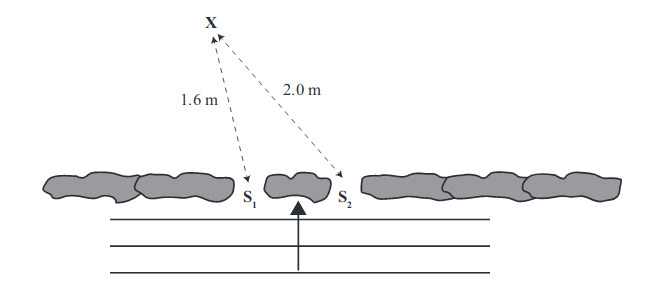
\includegraphics[width=0.5\textwidth]{nzqa20141}
    \question Water waves travel from deep to shallow water. The wave-fronts of the wave hit the boundary between the depths at
              a shallow angle. Draw a diagram showing the relation of the wavefronts leaving the boundary to those reaching it.
              Which phenomenon does your diagram illustrate?

              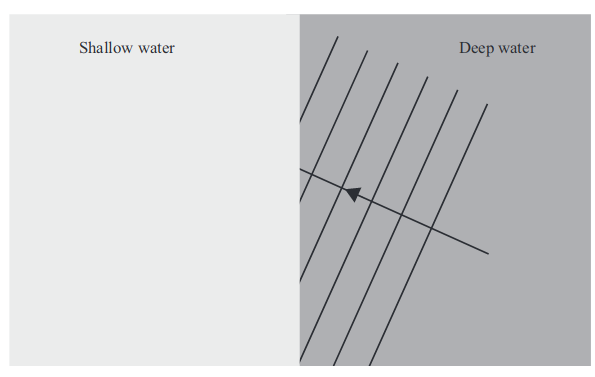
\includegraphics[width=0.5\textwidth]{nzqa20142}
    \question Consider the following systems of waves.

              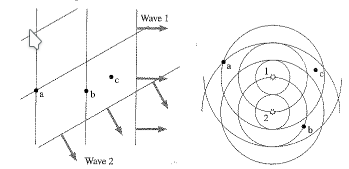
\includegraphics[width=0.5\textwidth]{knight1789}
      \begin{parts}
        \part In the left-hand system, both waves have an amplitude of \SI{2.0}{\milli\metre} and the same wavelength. What
              is the net displacement of the medium at points $ a $, $ b $, and $ c $?
        \part In the right-hand system, both circular waves are in phase. Are $ a $, $ b $, and $ c $ points of maximum constructive
              interference, points of maximum destructive interference, or in between?
      \end{parts}
    \question A water wave initially of wavelength \SI{3.0}{\centi\metre} and period \SI{0.50}{\second} enters
              water of a different depth where its speed is \SI{2.0}{\centi\metre\per\second}. Calculate the
              changed wavelength.
    \question Which of the following waves is diffracted most by an open square window of width \SI{0.5}{\metre}?
      \begin{parts}
        \part Microwaves of frequency \SI{10}{\giga\hertz} and speed \SI{3.0e8}{\metre\per\second}
        \part Light waves of wavelength \SI{650}{\nano\metre}
        \part Sound waves of frequency \SI{1050}{\hertz} and speed \SI{350}{\metre\per\second}
      \end{parts}
    \question Noise-cancelling headphones are an application of destructive interference. Each side of the headphones uses a microphone
              to pick up noise, delays it slightly, and then rebroadcasts it to your ear where it can interfere with the incoming sound
              wave of the noise. Suppose you are sitting \SI{1.5}{\metre} from an annoying \SI{120}{\hertz} buzzing sound. What is the
              minimum headphone delay, in milliseconds, that will cancel this noise?
  \end{questions}
  \subsection*{Section 1.5}
  \begin{questions}
    \question A boy \SI{1.5}{\metre} tall whose eyes are \SI{1.4}{\metre} from the floor when he stands
              straight can just see his complete image in a wall mirror.
      \begin{parts}
        \part What is the smallest length of the mirror that allows the boy to see his full length?
        \part How high off the ground is the mirror's bottom edge?
      \end{parts}

    \question An object \SI{1.5}{\centi\metre} high is placed \SI{2.5}{\centi\metre} in front of
              a concave mirror with a focal length of \SI{5.0}{\centi\metre}. Draw a ray diagram,
              and identify the nature of the image formed.

    \question An object \SI{2.0}{\centi\metre} high is placed \SI{12}{\centi\metre} in front of
              a concave mirror. The image formed is \SI{1}{\centi\metre} high. How far away from
              the mirror is the image formed?

    \question How far should an object be placed in front of a concave mirror with a radius of
              curvature \SI{36}{\centi\metre} in order to form a real image \SI{1}{9} of its size?

    \question It is possible to produce an image with a magnification of 2 when an object is \SI{12}{\centi\metre}
              away from the mirror. Find the focal length of the mirror if the image is virtual.

    \question A beam of light strikes a pool of water at a angle of incidence of \SI{60.0}{\degree}. Some light is
              reflected, and some is refracted. Find the directions of both the reflected and refracted rays, given
              that the index of refraction of water is $ n_w = 1.33 $.

    \question A beam of light moves from an unknown substance with a refractive index of $ n_1 = 1.33 $ into air. Supposing that the
              speed of light in air is $ \SI{2.99e8}{\metre\per\second} $, what is the speed of light in the unknown substance?

    \question Recall that the critical angle is the angle at which light is totally reflected back into the originating
              medium when it meets the boundary.
      \begin{parts}
        \part Give the condition(s) needed for total internal reflection to occur.
        \part If the exact critical angle for red light travelling from water into air is \SI{48.70}{\degree}, calculate the
              refractive index of water for red light.
      \end{parts}
    \question A person of height \SI{1.7}{\metre} is standing \SI{2}{\metre} from a concave mirror with a focal length of \SI{20}{\metre}.
              State the nature of the image formed, and give the magnification.
    \question A beam of light travels from a ruby ($ n = 1.76 $) into ice ($ n = 1.31 $).
      \begin{parts}
        \item The initial angle of incidence is \SI{30}{\degree}. If some light is refracted and some is
              reflected, find the angles of refraction and reflection.
        \item The angle of incidence is gradually increased. At what angle does light cease being refracted and totally reflect?
      \end{parts}
    \question A person of height \SI{1.7}{\metre} is standing \SI{2}{\metre} from a concave mirror with a focal length of \SI{20}{\metre}.
              State the nature of the image formed, and give the magnification.
    \question A beam of light travels from a ruby ($ n = 1.76 $) into ice ($ n = 1.31 $).
      \begin{parts}
        \item The initial angle of incidence is \SI{30}{\degree}. If some light is refracted and some is
              reflected, find the angles of refraction and reflection.
        \item The angle of incidence is gradually increased. At what angle does light cease being refracted and totally reflect?
      \end{parts}
    \question Large convex mirrors are often used in shops to improve security. Tracey
              is looking at herself in a convex security mirror of focal length \SI{2.0}{\metre}.
              Tracey is \SI{4.0}{\metre} away from the mirror, and is \SI{1.5}{\metre} tall.
              Draw a ray diagram and use it to calculate:
      \begin{parts}
        \part The position of Tracey's image.
        \part The size of Tracey's image.
      \end{parts}
    \question Find the position of the image of a candle flame located \SI{40}{\centi\metre} in
              front of a concave spherical mirror of radius of curvature \SI{64}{\centi\metre},
              and describe the type of image formed.
    \question An object and its image in a mirror are the same height when the object is \SI{36}{\centi\metre}
              from the mirror. What type of mirror is used, and what is its focal length?
    \question A ray of light passes from glass ($ n = 1.5 $) to air ($ n = 1.0 $).
      \begin{parts}
        \part Is the ray deflected towards the normal, or away from the normal?
        \part If the angle of incidence is \SI{50}{\degree}, what is the angle of refraction?
      \end{parts}
    \question A layer of oil ($ n = 1.45 $) floats on water ($ n = 1.33 $). A ray of light shines into the oil
              with an angle of incidence of \SI{40.0}{\degree}.
      \begin{parts}
        \part Draw a diagram of the system, and label the angle of refraction $ \theta $ of the light in the water.
        \part Calculate the value of $ \theta $.
      \end{parts}
    \question The refractive index of diamond is $ n = 2.42 $.
      \begin{parts}
        \item Can total internal reflection occur if light is passes from air into the diamond? Explain.
        \item What is the critical angle for light passing from diamond to air?
      \end{parts}
    \question By ray diagram or otherwise, find the position and magnification of the image formed by a convex lens of
              focal length \SI{100.0}{\centi\metre}, when the object is
      \begin{parts}
        \part \SI{150.0}{\centi\metre} from the lens.
        \part \SI{75.0}{\centi\metre} from the lens.
      \end{parts}
  \end{questions}
  \clearpage
  \section*{Formulae}
  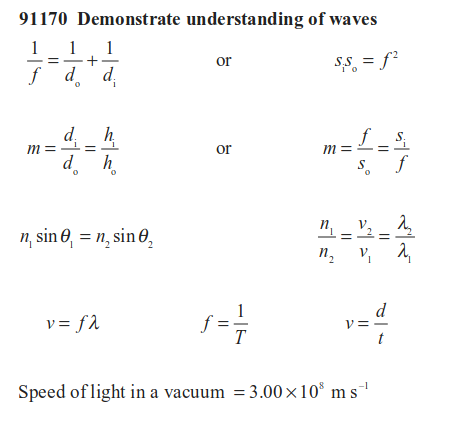
\includegraphics{waves}
\end{document}
